%!TEX root = ../thesis-main.tex
\chapter{Design}

\section{Architettura e macrostruttura}

Alchemist, come esplicato nella sezione 1.4, è un progetto modulare complesso in continuo sviluppo. Gli strumenti presentati nel capitolo precedente trovano già impiego nel progetto, ad eccezione del software di impacchettamento il quale è oggetto di questo elaborato. Per conseguire gli obiettivi del progetto è necessario coordinare i tre componenti che costituiscono la macrostruttura del progetto. I tre componenti si possono distinguere come segue:
\begin{itemize}
	\item \textbf{Pipeline}: il flusso automatico gestito dall'infrastruttura di GitHub Actions. Questo componente è già presente e necessità quindi un aggiornamento per soddisfare i requisiti di questo elaborato.
	\item \textbf{Build system}: l'insieme dei processi e delle funzioni adibite alla produzione di artefatti utilizzando il software Gradle. Questo componente richiede lo sviluppo di nuovi task per la produzione dei pacchetti di installazione.
	\item \textbf{Release}: l'insieme dei requisiti per la pubblicazione nei repository pubblici come \ac{aur}. Questo componente sfrutterà i due componenti precedenti per costruire i pacchetti ed i metadati nel rispetto delle regole che il repository pubblico emana.
\end{itemize}

\subsection{Pipeline}

Alchemist utilizza fondamentalmente due workflow per soddisfare i requisiti di integrazione e rilascio continuo. Un primo workflow chiamato ``dispatcher", il quale funziona come punto di inizio del flusso, è in ascolto di eventi e una volta avviato esamina (inspect) i meta-dati dell'evento scatenante per determinare lo step successivo. In particolare nella configurazione in oggetto questo step iniziale funge da filtro dal momento che esiste un solo possibile step successivo, ossia il secondo workflow quello adibito a soddisfare i compiti di build, test e distribuzione.
Per compiere le tre funzioni il workflow è formato dai seguenti job.
\begin{itemize}
	\item \textbf{select-java-version}: è il punto di inizio ed ha il compito di propagare la versione minima supportata di Java per replicare lo stesso ambiente \ac{jre} nei successivi job.
	\item \textbf{build}: esegue un'analisi statica del codice e gli unit test. Utilizza una strategia a matrice per costruire più istanze in ambienti diversi: in questo caso nei tre sistemi operativi principali. 
	\item \textbf{test-deploy}: esegue un test del deploy dei moduli di Alchemist. Il test è strettamente necessario per l'esecuzione corretta di un rilascio.
	\item \textbf{build-website}: costruisce il sito web di documentazione e lo prepara per il rilascio.
	\item \textbf{release}: analizza attraverso tecniche di semantic-versioning se è necessario il rilascio di una nuova versione del software. In caso positivo: costruisce i JAR, ottiene il sito e pubblica una nuova versione.
	\item \textbf{success}: infine, controlla che l'output di ogni job sia esente da errori.
\end{itemize}

\paragraph{Workflow risultante} La nuova pipeline, descritta in figura 3.2, introduce due job all'interno del flusso cercando di sfruttare il più possibile la computazione parallela per ottimizzare i tempi di esecuzione.
\begin{figure}[H]
	\centering
	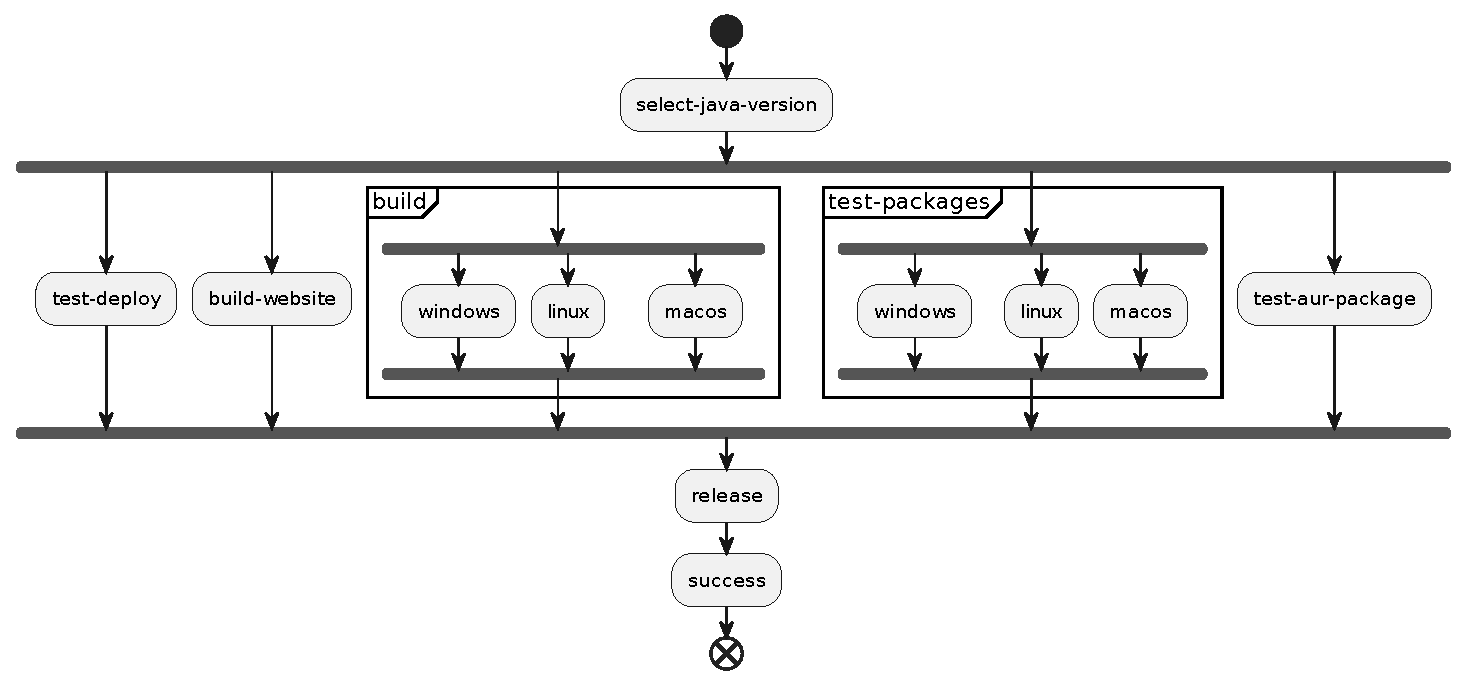
\includegraphics[width=1\linewidth]{figures/activity-diagram-pipeline.pdf}
	\caption{Diagramma dell'attività illustrante la pipeline}
	\label{fig:activity-diagram-pipeline}
\end{figure}
Mentre per la generazione ed il rilascio esistono già dei job adibiti, è buona norma configurare singoli job riservati al test di una particolare funzionalità, in modo che il test venga eseguito in un ambiente basilare senza potenziali modifiche che possono interferire con l'esito. Il comportamento di default dei job all'interno della pipeline è bloccante per cui il fallimento di un test porta all'interruzione dell'intera pipeline.

\begin{figure}[H]
	\centering
	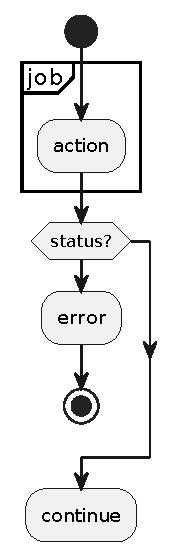
\includegraphics[width=.13\linewidth]{figures/activity-diagram-job.pdf}
	\caption{Diagramma dell'attività illustrante il comportamento dei job all'interno della pipeline}
	\label{fig:activity-diagram-job}
\end{figure}

Il primo job \texttt{test-packages} utilizza la strategia a matrice per eseguire la procedura sui tre sistemi operativi target del progetto ed ha il compito di generare e controllare la validità dei pacchetti di installazione. Il secondo \texttt{test-aur-package} installa localmente il pacchetto all'interno di un container \textit{arch-linux} ed infine controlla il corretto esito dell'operazione costruendo il pacchetto con \textit{makepkg} ed installandolo con \textit{pacman}.

\subsection{Build system}

Il ruolo del \textit{build system} è quello di esporre un \textit{task} adibito alla generazione dei pacchetti utilizzando \textit{jpackage}. Come discusso nel capitolo precedente, \textit{jpackage} offre un'interfaccia \ac{cli} con diverse opzioni per configurare e personalizzare a piacimento i pacchetti in output. Esistono parametri generici, compatibili con tutte le piattaforme, e parametri specifici che vanno a modificare attributi particolari alla tipologia di pacchetto in output scelta.

\paragraph{jpackage} Uno dei motivi che ha portato alla scelta di \textit{jpackage} rispetto ad altri software è la capacità di includere autonomamente una \textit{runtime-image} di Java ossia una \ac{jre} ridotta di dimensioni all'interno del pacchetto. La combinazione di una \textit{runtime-image} e degli archivi Java (JAR) necessari all'esecuzione dell'applicazione costituiscono l'\textit{application-image}: un pacchetto autocontenuto che include l'applicazione, assieme una \ac{jvm} ed alle librerie necessarie per eseguire quell'applicazione sulla piattaforma di destinazione. La generazione della \textit{runtime-image}, se non inclusa manualmente, è delegata ad uno strumento del jdk di nome \textit{jlink}.

Alchemist, come specificato nella documentazione\footnote{https://alchemistsimulator.github.io/howtos/preparation/jar/index.html}, può essere avviato in modalità stand-alone utilizzando l'archivio denominato ``full". L'\textit{application-image} finale è formato come descritto nella figura 3.3.

\begin{figure}[H]
	\centering
	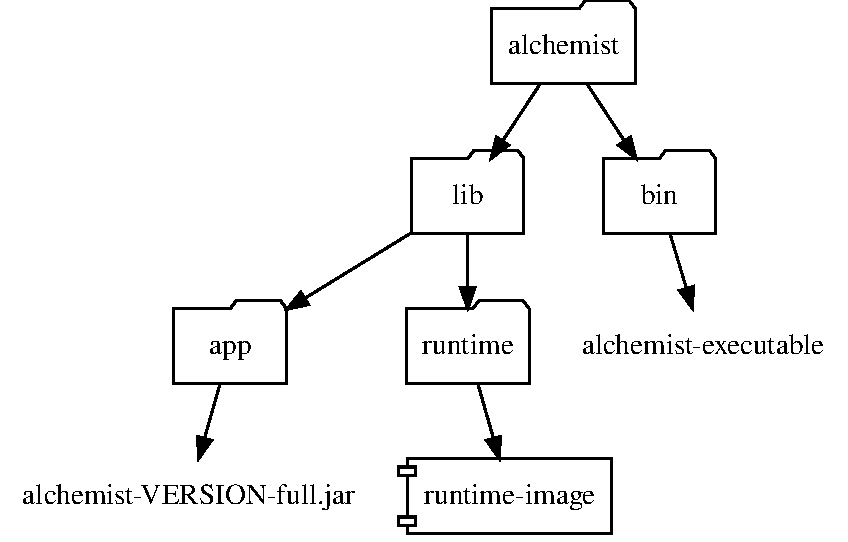
\includegraphics[width=.7\linewidth]{figures/application-image-folder-structure.pdf}
	\caption{Struttura del filesystem dell'\textit{application image} generato da \textit{jpackage}}
	\label{fig:activity-diagram-job}
\end{figure}

\paragraph{Plugin Gradle}


\subsection{Release}
Citare wiki, citare le regole, capire come ovviare alle regole